\section{Actividad No 03 – Apache Allura} 
Allura es un software de código abierto de Apache para la gestión de repositorios de código fuente, informes de errores, debates, páginas wiki, blogs y otros contenidos online. Para llevar a cabo el seguimiento de incidentes en Allura puedes recurrir tanto a las opciones de formateo y archivos adjuntos de Markdown como a los tickets provistos por el sistema llamado Milestones. Asimismo, también hay disponible una sintaxis de búsqueda avanzada con la que, por ejemplo, se pueden guardar las consultas más frecuentes. Sin embargo, Apache Allura no permite el análisis del código. La plataforma, además, fue desarrollada con el lenguaje de programación Python.

\begin{itemize}


           \item\textbf {Caracteristicas}
           \item\textbf {Seguimiento de Problemas}
            El seguimiento de problemas en Allura ha sido repensado desde cero. Usamos nuestro propio seguimiento de problemas en el desarrollo de Allura (¡Allura está completamente alojada en uno mismo!) Por lo que estamos obligados a pensar en el proceso a diario.

           \item\textbf {Documentación}
            Ayudar a los usuarios a usar su producto es tan importante como hacerlo en primer lugar. Entonces ofrecemos varias formas diferentes de crear su documentación. Comenzamos con una wiki, pero puede instalar y usar cualquier herramienta que desee en el espacio web de su proyecto.

            \item\textbf {Codigo Abierto}
            Como si todo eso no fuera suficiente, Allura es de código abierto y se lanzó bajo la licencia de Apache. Puede descargarlo, alojar su propia fragua y realizar mejoras en el código. Nos encantaría que participaras en el establecimiento del futuro desarrollo de Allura. Si eres programador, diseñador, experto en UI / UX de Python, o tienes otras habilidades con las que puedes contribuir al esfuerzo, salta y ocupate.
	

           \item\textbf {Cuadro de comparacion}

	El cuadro a continuación ofrece una comparación de características entre Allura y varias otras plataformas de software de forjado de código abierto.

	\begin{center}
	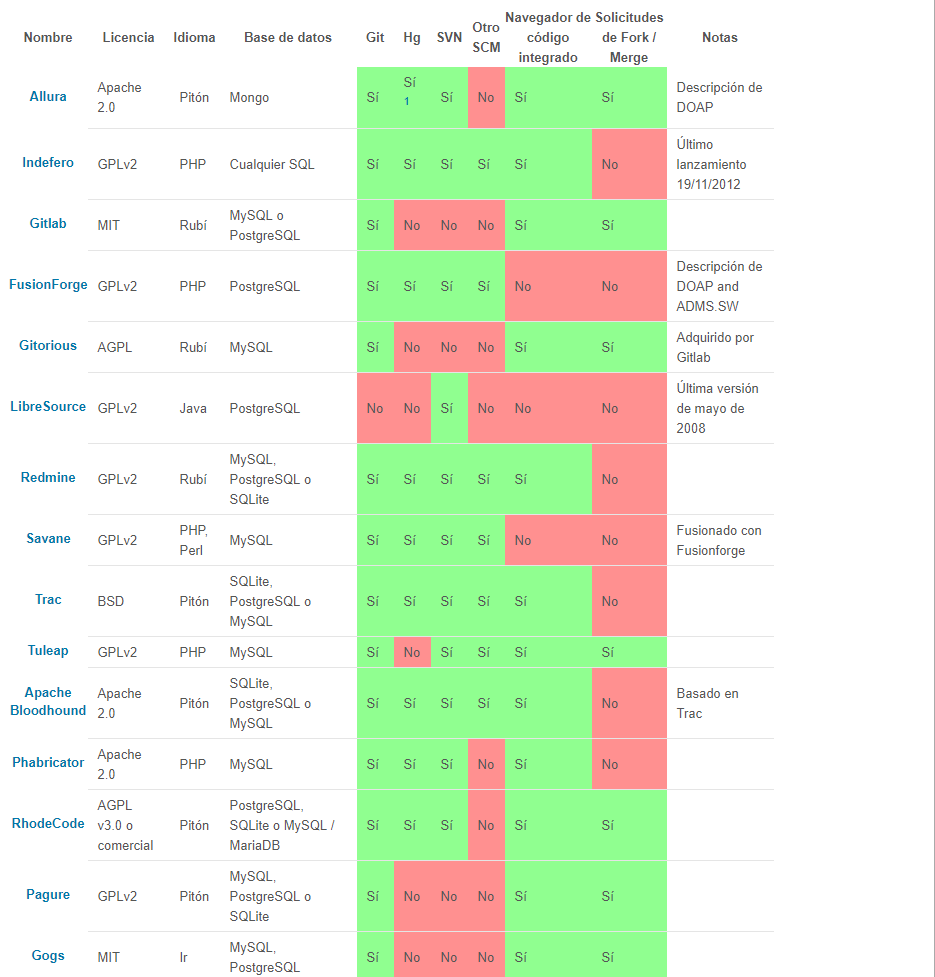
\includegraphics[width=17cm]{./Imagenes/cuadro1} 
	\end{center}

       


\end{itemize} 